\documentclass[tikz,border=8pt]{standalone}
\usepackage{amsmath}
\usetikzlibrary{arrows.meta,calc,decorations.pathmorphing}
\definecolor{ink}{HTML}{17324D}
\definecolor{accent}{HTML}{0F766E}
\definecolor{gold}{HTML}{C28524}
\begin{document}
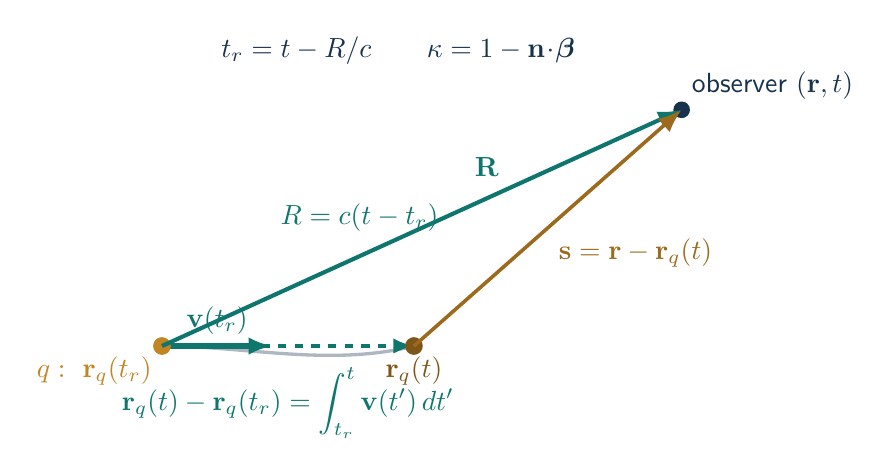
\begin{tikzpicture}[>=Latex,font=\sffamily,thick]
  \def\pathx#1{-2.2+3.2*(#1)}
  \def\pathy#1{-.8*(#1)*(#1)*(1-(#1))}
  \coordinate (Qr) at ({\pathx{0}},{\pathy{0}});
  \coordinate (Qn) at ({\pathx{1}},{\pathy{1}});
  \coordinate (P) at (4.4,3.0);
  \draw[ink!35,line width=1.2pt]
    plot[domain=0:1,samples=101]
    ({\pathx{\x}},{\pathy{\x}});
  \draw[accent,line width=2pt,-{Latex[length=3mm]}] (Qr) -- ($(Qr)+(1.4,0)$)
    node[midway,above] {$\mathbf v(t_r)$};
  \draw[accent,dashed,line width=1.2pt,-{Latex[length=2.6mm]}] (Qr) -- (Qn)
    node[midway,below=4pt]
    {$\displaystyle \mathbf r_q(t)-\mathbf r_q(t_r)
      =\int_{t_r}^{t}\mathbf v(t')\,dt'$};
  \fill[gold] (Qr) circle (3.2pt) node[below left] {$q:\ \mathbf r_q(t_r)$};
  \fill[gold!65!black] (Qn) circle (3.2pt) node[below] {$\mathbf r_q(t)$};
  \fill[ink] (P) circle (3pt) node[above right] {observer $(\mathbf r,t)$};
  \draw[accent,-{Latex[length=3mm]},line width=1.5pt] (Qr) -- (P)
    node[pos=.67,above left] {$\mathbf R$}
    node[pos=.38,above=5pt] {$R=c(t-t_r)$};
  \draw[gold!80!black,-{Latex[length=3mm]},line width=1.3pt] (Qn) -- (P)
    node[midway,below right] {$\mathbf s=\mathbf r-\mathbf r_q(t)$};
  \node[align=center,ink] at (0.8,3.75)
    {$t_r=t-R/c$\qquad $\kappa=1-\mathbf n\!\cdot\!\boldsymbol\beta$};
\end{tikzpicture}
\end{document}
